
    




    
\documentclass[11pt]{article}

    
    \usepackage[breakable]{tcolorbox}
    \tcbset{nobeforeafter} % prevents tcolorboxes being placing in paragraphs
    \usepackage{float}
    \floatplacement{figure}{H} % forces figures to be placed at the correct location
    
    \usepackage[T1]{fontenc}
    % Nicer default font (+ math font) than Computer Modern for most use cases
    \usepackage{mathpazo}

    % Basic figure setup, for now with no caption control since it's done
    % automatically by Pandoc (which extracts ![](path) syntax from Markdown).
    \usepackage{graphicx}
    % We will generate all images so they have a width \maxwidth. This means
    % that they will get their normal width if they fit onto the page, but
    % are scaled down if they would overflow the margins.
    \makeatletter
    \def\maxwidth{\ifdim\Gin@nat@width>\linewidth\linewidth
    \else\Gin@nat@width\fi}
    \makeatother
    \let\Oldincludegraphics\includegraphics
    % Set max figure width to be 80% of text width, for now hardcoded.
    \renewcommand{\includegraphics}[1]{\Oldincludegraphics[width=.8\maxwidth]{#1}}
    % Ensure that by default, figures have no caption (until we provide a
    % proper Figure object with a Caption API and a way to capture that
    % in the conversion process - todo).
    \usepackage{caption}
    \DeclareCaptionLabelFormat{nolabel}{}
    \captionsetup{labelformat=nolabel}

    \usepackage{adjustbox} % Used to constrain images to a maximum size 
    \usepackage{xcolor} % Allow colors to be defined
    \usepackage{enumerate} % Needed for markdown enumerations to work
    \usepackage{geometry} % Used to adjust the document margins
    \usepackage{amsmath} % Equations
    \usepackage{amssymb} % Equations
    \usepackage{textcomp} % defines textquotesingle
    % Hack from http://tex.stackexchange.com/a/47451/13684:
    \AtBeginDocument{%
        \def\PYZsq{\textquotesingle}% Upright quotes in Pygmentized code
    }
    \usepackage{upquote} % Upright quotes for verbatim code
    \usepackage{eurosym} % defines \euro
    \usepackage[mathletters]{ucs} % Extended unicode (utf-8) support
    \usepackage[utf8x]{inputenc} % Allow utf-8 characters in the tex document
    \usepackage{fancyvrb} % verbatim replacement that allows latex
    \usepackage{grffile} % extends the file name processing of package graphics 
                         % to support a larger range 
    % The hyperref package gives us a pdf with properly built
    % internal navigation ('pdf bookmarks' for the table of contents,
    % internal cross-reference links, web links for URLs, etc.)
    \usepackage{hyperref}
    \usepackage{longtable} % longtable support required by pandoc >1.10
    \usepackage{booktabs}  % table support for pandoc > 1.12.2
    \usepackage[inline]{enumitem} % IRkernel/repr support (it uses the enumerate* environment)
    \usepackage[normalem]{ulem} % ulem is needed to support strikethroughs (\sout)
                                % normalem makes italics be italics, not underlines
    \usepackage{mathrsfs}
    

    
    % Colors for the hyperref package
    \definecolor{urlcolor}{rgb}{0,.145,.698}
    \definecolor{linkcolor}{rgb}{.71,0.21,0.01}
    \definecolor{citecolor}{rgb}{.12,.54,.11}

    % ANSI colors
    \definecolor{ansi-black}{HTML}{3E424D}
    \definecolor{ansi-black-intense}{HTML}{282C36}
    \definecolor{ansi-red}{HTML}{E75C58}
    \definecolor{ansi-red-intense}{HTML}{B22B31}
    \definecolor{ansi-green}{HTML}{00A250}
    \definecolor{ansi-green-intense}{HTML}{007427}
    \definecolor{ansi-yellow}{HTML}{DDB62B}
    \definecolor{ansi-yellow-intense}{HTML}{B27D12}
    \definecolor{ansi-blue}{HTML}{208FFB}
    \definecolor{ansi-blue-intense}{HTML}{0065CA}
    \definecolor{ansi-magenta}{HTML}{D160C4}
    \definecolor{ansi-magenta-intense}{HTML}{A03196}
    \definecolor{ansi-cyan}{HTML}{60C6C8}
    \definecolor{ansi-cyan-intense}{HTML}{258F8F}
    \definecolor{ansi-white}{HTML}{C5C1B4}
    \definecolor{ansi-white-intense}{HTML}{A1A6B2}
    \definecolor{ansi-default-inverse-fg}{HTML}{FFFFFF}
    \definecolor{ansi-default-inverse-bg}{HTML}{000000}

    % commands and environments needed by pandoc snippets
    % extracted from the output of `pandoc -s`
    \providecommand{\tightlist}{%
      \setlength{\itemsep}{0pt}\setlength{\parskip}{0pt}}
    \DefineVerbatimEnvironment{Highlighting}{Verbatim}{commandchars=\\\{\}}
    % Add ',fontsize=\small' for more characters per line
    \newenvironment{Shaded}{}{}
    \newcommand{\KeywordTok}[1]{\textcolor[rgb]{0.00,0.44,0.13}{\textbf{{#1}}}}
    \newcommand{\DataTypeTok}[1]{\textcolor[rgb]{0.56,0.13,0.00}{{#1}}}
    \newcommand{\DecValTok}[1]{\textcolor[rgb]{0.25,0.63,0.44}{{#1}}}
    \newcommand{\BaseNTok}[1]{\textcolor[rgb]{0.25,0.63,0.44}{{#1}}}
    \newcommand{\FloatTok}[1]{\textcolor[rgb]{0.25,0.63,0.44}{{#1}}}
    \newcommand{\CharTok}[1]{\textcolor[rgb]{0.25,0.44,0.63}{{#1}}}
    \newcommand{\StringTok}[1]{\textcolor[rgb]{0.25,0.44,0.63}{{#1}}}
    \newcommand{\CommentTok}[1]{\textcolor[rgb]{0.38,0.63,0.69}{\textit{{#1}}}}
    \newcommand{\OtherTok}[1]{\textcolor[rgb]{0.00,0.44,0.13}{{#1}}}
    \newcommand{\AlertTok}[1]{\textcolor[rgb]{1.00,0.00,0.00}{\textbf{{#1}}}}
    \newcommand{\FunctionTok}[1]{\textcolor[rgb]{0.02,0.16,0.49}{{#1}}}
    \newcommand{\RegionMarkerTok}[1]{{#1}}
    \newcommand{\ErrorTok}[1]{\textcolor[rgb]{1.00,0.00,0.00}{\textbf{{#1}}}}
    \newcommand{\NormalTok}[1]{{#1}}
    
    % Additional commands for more recent versions of Pandoc
    \newcommand{\ConstantTok}[1]{\textcolor[rgb]{0.53,0.00,0.00}{{#1}}}
    \newcommand{\SpecialCharTok}[1]{\textcolor[rgb]{0.25,0.44,0.63}{{#1}}}
    \newcommand{\VerbatimStringTok}[1]{\textcolor[rgb]{0.25,0.44,0.63}{{#1}}}
    \newcommand{\SpecialStringTok}[1]{\textcolor[rgb]{0.73,0.40,0.53}{{#1}}}
    \newcommand{\ImportTok}[1]{{#1}}
    \newcommand{\DocumentationTok}[1]{\textcolor[rgb]{0.73,0.13,0.13}{\textit{{#1}}}}
    \newcommand{\AnnotationTok}[1]{\textcolor[rgb]{0.38,0.63,0.69}{\textbf{\textit{{#1}}}}}
    \newcommand{\CommentVarTok}[1]{\textcolor[rgb]{0.38,0.63,0.69}{\textbf{\textit{{#1}}}}}
    \newcommand{\VariableTok}[1]{\textcolor[rgb]{0.10,0.09,0.49}{{#1}}}
    \newcommand{\ControlFlowTok}[1]{\textcolor[rgb]{0.00,0.44,0.13}{\textbf{{#1}}}}
    \newcommand{\OperatorTok}[1]{\textcolor[rgb]{0.40,0.40,0.40}{{#1}}}
    \newcommand{\BuiltInTok}[1]{{#1}}
    \newcommand{\ExtensionTok}[1]{{#1}}
    \newcommand{\PreprocessorTok}[1]{\textcolor[rgb]{0.74,0.48,0.00}{{#1}}}
    \newcommand{\AttributeTok}[1]{\textcolor[rgb]{0.49,0.56,0.16}{{#1}}}
    \newcommand{\InformationTok}[1]{\textcolor[rgb]{0.38,0.63,0.69}{\textbf{\textit{{#1}}}}}
    \newcommand{\WarningTok}[1]{\textcolor[rgb]{0.38,0.63,0.69}{\textbf{\textit{{#1}}}}}
    
    
    % Define a nice break command that doesn't care if a line doesn't already
    % exist.
    \def\br{\hspace*{\fill} \\* }
    % Math Jax compatibility definitions
    \def\gt{>}
    \def\lt{<}
    \let\Oldtex\TeX
    \let\Oldlatex\LaTeX
    \renewcommand{\TeX}{\textrm{\Oldtex}}
    \renewcommand{\LaTeX}{\textrm{\Oldlatex}}
    % Document parameters
    % Document title
    \title{report}
    
    
    
    
    
% Pygments definitions
\makeatletter
\def\PY@reset{\let\PY@it=\relax \let\PY@bf=\relax%
    \let\PY@ul=\relax \let\PY@tc=\relax%
    \let\PY@bc=\relax \let\PY@ff=\relax}
\def\PY@tok#1{\csname PY@tok@#1\endcsname}
\def\PY@toks#1+{\ifx\relax#1\empty\else%
    \PY@tok{#1}\expandafter\PY@toks\fi}
\def\PY@do#1{\PY@bc{\PY@tc{\PY@ul{%
    \PY@it{\PY@bf{\PY@ff{#1}}}}}}}
\def\PY#1#2{\PY@reset\PY@toks#1+\relax+\PY@do{#2}}

\expandafter\def\csname PY@tok@w\endcsname{\def\PY@tc##1{\textcolor[rgb]{0.73,0.73,0.73}{##1}}}
\expandafter\def\csname PY@tok@c\endcsname{\let\PY@it=\textit\def\PY@tc##1{\textcolor[rgb]{0.25,0.50,0.50}{##1}}}
\expandafter\def\csname PY@tok@cp\endcsname{\def\PY@tc##1{\textcolor[rgb]{0.74,0.48,0.00}{##1}}}
\expandafter\def\csname PY@tok@k\endcsname{\let\PY@bf=\textbf\def\PY@tc##1{\textcolor[rgb]{0.00,0.50,0.00}{##1}}}
\expandafter\def\csname PY@tok@kp\endcsname{\def\PY@tc##1{\textcolor[rgb]{0.00,0.50,0.00}{##1}}}
\expandafter\def\csname PY@tok@kt\endcsname{\def\PY@tc##1{\textcolor[rgb]{0.69,0.00,0.25}{##1}}}
\expandafter\def\csname PY@tok@o\endcsname{\def\PY@tc##1{\textcolor[rgb]{0.40,0.40,0.40}{##1}}}
\expandafter\def\csname PY@tok@ow\endcsname{\let\PY@bf=\textbf\def\PY@tc##1{\textcolor[rgb]{0.67,0.13,1.00}{##1}}}
\expandafter\def\csname PY@tok@nb\endcsname{\def\PY@tc##1{\textcolor[rgb]{0.00,0.50,0.00}{##1}}}
\expandafter\def\csname PY@tok@nf\endcsname{\def\PY@tc##1{\textcolor[rgb]{0.00,0.00,1.00}{##1}}}
\expandafter\def\csname PY@tok@nc\endcsname{\let\PY@bf=\textbf\def\PY@tc##1{\textcolor[rgb]{0.00,0.00,1.00}{##1}}}
\expandafter\def\csname PY@tok@nn\endcsname{\let\PY@bf=\textbf\def\PY@tc##1{\textcolor[rgb]{0.00,0.00,1.00}{##1}}}
\expandafter\def\csname PY@tok@ne\endcsname{\let\PY@bf=\textbf\def\PY@tc##1{\textcolor[rgb]{0.82,0.25,0.23}{##1}}}
\expandafter\def\csname PY@tok@nv\endcsname{\def\PY@tc##1{\textcolor[rgb]{0.10,0.09,0.49}{##1}}}
\expandafter\def\csname PY@tok@no\endcsname{\def\PY@tc##1{\textcolor[rgb]{0.53,0.00,0.00}{##1}}}
\expandafter\def\csname PY@tok@nl\endcsname{\def\PY@tc##1{\textcolor[rgb]{0.63,0.63,0.00}{##1}}}
\expandafter\def\csname PY@tok@ni\endcsname{\let\PY@bf=\textbf\def\PY@tc##1{\textcolor[rgb]{0.60,0.60,0.60}{##1}}}
\expandafter\def\csname PY@tok@na\endcsname{\def\PY@tc##1{\textcolor[rgb]{0.49,0.56,0.16}{##1}}}
\expandafter\def\csname PY@tok@nt\endcsname{\let\PY@bf=\textbf\def\PY@tc##1{\textcolor[rgb]{0.00,0.50,0.00}{##1}}}
\expandafter\def\csname PY@tok@nd\endcsname{\def\PY@tc##1{\textcolor[rgb]{0.67,0.13,1.00}{##1}}}
\expandafter\def\csname PY@tok@s\endcsname{\def\PY@tc##1{\textcolor[rgb]{0.73,0.13,0.13}{##1}}}
\expandafter\def\csname PY@tok@sd\endcsname{\let\PY@it=\textit\def\PY@tc##1{\textcolor[rgb]{0.73,0.13,0.13}{##1}}}
\expandafter\def\csname PY@tok@si\endcsname{\let\PY@bf=\textbf\def\PY@tc##1{\textcolor[rgb]{0.73,0.40,0.53}{##1}}}
\expandafter\def\csname PY@tok@se\endcsname{\let\PY@bf=\textbf\def\PY@tc##1{\textcolor[rgb]{0.73,0.40,0.13}{##1}}}
\expandafter\def\csname PY@tok@sr\endcsname{\def\PY@tc##1{\textcolor[rgb]{0.73,0.40,0.53}{##1}}}
\expandafter\def\csname PY@tok@ss\endcsname{\def\PY@tc##1{\textcolor[rgb]{0.10,0.09,0.49}{##1}}}
\expandafter\def\csname PY@tok@sx\endcsname{\def\PY@tc##1{\textcolor[rgb]{0.00,0.50,0.00}{##1}}}
\expandafter\def\csname PY@tok@m\endcsname{\def\PY@tc##1{\textcolor[rgb]{0.40,0.40,0.40}{##1}}}
\expandafter\def\csname PY@tok@gh\endcsname{\let\PY@bf=\textbf\def\PY@tc##1{\textcolor[rgb]{0.00,0.00,0.50}{##1}}}
\expandafter\def\csname PY@tok@gu\endcsname{\let\PY@bf=\textbf\def\PY@tc##1{\textcolor[rgb]{0.50,0.00,0.50}{##1}}}
\expandafter\def\csname PY@tok@gd\endcsname{\def\PY@tc##1{\textcolor[rgb]{0.63,0.00,0.00}{##1}}}
\expandafter\def\csname PY@tok@gi\endcsname{\def\PY@tc##1{\textcolor[rgb]{0.00,0.63,0.00}{##1}}}
\expandafter\def\csname PY@tok@gr\endcsname{\def\PY@tc##1{\textcolor[rgb]{1.00,0.00,0.00}{##1}}}
\expandafter\def\csname PY@tok@ge\endcsname{\let\PY@it=\textit}
\expandafter\def\csname PY@tok@gs\endcsname{\let\PY@bf=\textbf}
\expandafter\def\csname PY@tok@gp\endcsname{\let\PY@bf=\textbf\def\PY@tc##1{\textcolor[rgb]{0.00,0.00,0.50}{##1}}}
\expandafter\def\csname PY@tok@go\endcsname{\def\PY@tc##1{\textcolor[rgb]{0.53,0.53,0.53}{##1}}}
\expandafter\def\csname PY@tok@gt\endcsname{\def\PY@tc##1{\textcolor[rgb]{0.00,0.27,0.87}{##1}}}
\expandafter\def\csname PY@tok@err\endcsname{\def\PY@bc##1{\setlength{\fboxsep}{0pt}\fcolorbox[rgb]{1.00,0.00,0.00}{1,1,1}{\strut ##1}}}
\expandafter\def\csname PY@tok@kc\endcsname{\let\PY@bf=\textbf\def\PY@tc##1{\textcolor[rgb]{0.00,0.50,0.00}{##1}}}
\expandafter\def\csname PY@tok@kd\endcsname{\let\PY@bf=\textbf\def\PY@tc##1{\textcolor[rgb]{0.00,0.50,0.00}{##1}}}
\expandafter\def\csname PY@tok@kn\endcsname{\let\PY@bf=\textbf\def\PY@tc##1{\textcolor[rgb]{0.00,0.50,0.00}{##1}}}
\expandafter\def\csname PY@tok@kr\endcsname{\let\PY@bf=\textbf\def\PY@tc##1{\textcolor[rgb]{0.00,0.50,0.00}{##1}}}
\expandafter\def\csname PY@tok@bp\endcsname{\def\PY@tc##1{\textcolor[rgb]{0.00,0.50,0.00}{##1}}}
\expandafter\def\csname PY@tok@fm\endcsname{\def\PY@tc##1{\textcolor[rgb]{0.00,0.00,1.00}{##1}}}
\expandafter\def\csname PY@tok@vc\endcsname{\def\PY@tc##1{\textcolor[rgb]{0.10,0.09,0.49}{##1}}}
\expandafter\def\csname PY@tok@vg\endcsname{\def\PY@tc##1{\textcolor[rgb]{0.10,0.09,0.49}{##1}}}
\expandafter\def\csname PY@tok@vi\endcsname{\def\PY@tc##1{\textcolor[rgb]{0.10,0.09,0.49}{##1}}}
\expandafter\def\csname PY@tok@vm\endcsname{\def\PY@tc##1{\textcolor[rgb]{0.10,0.09,0.49}{##1}}}
\expandafter\def\csname PY@tok@sa\endcsname{\def\PY@tc##1{\textcolor[rgb]{0.73,0.13,0.13}{##1}}}
\expandafter\def\csname PY@tok@sb\endcsname{\def\PY@tc##1{\textcolor[rgb]{0.73,0.13,0.13}{##1}}}
\expandafter\def\csname PY@tok@sc\endcsname{\def\PY@tc##1{\textcolor[rgb]{0.73,0.13,0.13}{##1}}}
\expandafter\def\csname PY@tok@dl\endcsname{\def\PY@tc##1{\textcolor[rgb]{0.73,0.13,0.13}{##1}}}
\expandafter\def\csname PY@tok@s2\endcsname{\def\PY@tc##1{\textcolor[rgb]{0.73,0.13,0.13}{##1}}}
\expandafter\def\csname PY@tok@sh\endcsname{\def\PY@tc##1{\textcolor[rgb]{0.73,0.13,0.13}{##1}}}
\expandafter\def\csname PY@tok@s1\endcsname{\def\PY@tc##1{\textcolor[rgb]{0.73,0.13,0.13}{##1}}}
\expandafter\def\csname PY@tok@mb\endcsname{\def\PY@tc##1{\textcolor[rgb]{0.40,0.40,0.40}{##1}}}
\expandafter\def\csname PY@tok@mf\endcsname{\def\PY@tc##1{\textcolor[rgb]{0.40,0.40,0.40}{##1}}}
\expandafter\def\csname PY@tok@mh\endcsname{\def\PY@tc##1{\textcolor[rgb]{0.40,0.40,0.40}{##1}}}
\expandafter\def\csname PY@tok@mi\endcsname{\def\PY@tc##1{\textcolor[rgb]{0.40,0.40,0.40}{##1}}}
\expandafter\def\csname PY@tok@il\endcsname{\def\PY@tc##1{\textcolor[rgb]{0.40,0.40,0.40}{##1}}}
\expandafter\def\csname PY@tok@mo\endcsname{\def\PY@tc##1{\textcolor[rgb]{0.40,0.40,0.40}{##1}}}
\expandafter\def\csname PY@tok@ch\endcsname{\let\PY@it=\textit\def\PY@tc##1{\textcolor[rgb]{0.25,0.50,0.50}{##1}}}
\expandafter\def\csname PY@tok@cm\endcsname{\let\PY@it=\textit\def\PY@tc##1{\textcolor[rgb]{0.25,0.50,0.50}{##1}}}
\expandafter\def\csname PY@tok@cpf\endcsname{\let\PY@it=\textit\def\PY@tc##1{\textcolor[rgb]{0.25,0.50,0.50}{##1}}}
\expandafter\def\csname PY@tok@c1\endcsname{\let\PY@it=\textit\def\PY@tc##1{\textcolor[rgb]{0.25,0.50,0.50}{##1}}}
\expandafter\def\csname PY@tok@cs\endcsname{\let\PY@it=\textit\def\PY@tc##1{\textcolor[rgb]{0.25,0.50,0.50}{##1}}}

\def\PYZbs{\char`\\}
\def\PYZus{\char`\_}
\def\PYZob{\char`\{}
\def\PYZcb{\char`\}}
\def\PYZca{\char`\^}
\def\PYZam{\char`\&}
\def\PYZlt{\char`\<}
\def\PYZgt{\char`\>}
\def\PYZsh{\char`\#}
\def\PYZpc{\char`\%}
\def\PYZdl{\char`\$}
\def\PYZhy{\char`\-}
\def\PYZsq{\char`\'}
\def\PYZdq{\char`\"}
\def\PYZti{\char`\~}
% for compatibility with earlier versions
\def\PYZat{@}
\def\PYZlb{[}
\def\PYZrb{]}
\makeatother


    % For linebreaks inside Verbatim environment from package fancyvrb. 
    \makeatletter
        \newbox\Wrappedcontinuationbox 
        \newbox\Wrappedvisiblespacebox 
        \newcommand*\Wrappedvisiblespace {\textcolor{red}{\textvisiblespace}} 
        \newcommand*\Wrappedcontinuationsymbol {\textcolor{red}{\llap{\tiny$\m@th\hookrightarrow$}}} 
        \newcommand*\Wrappedcontinuationindent {3ex } 
        \newcommand*\Wrappedafterbreak {\kern\Wrappedcontinuationindent\copy\Wrappedcontinuationbox} 
        % Take advantage of the already applied Pygments mark-up to insert 
        % potential linebreaks for TeX processing. 
        %        {, <, #, %, $, ' and ": go to next line. 
        %        _, }, ^, &, >, - and ~: stay at end of broken line. 
        % Use of \textquotesingle for straight quote. 
        \newcommand*\Wrappedbreaksatspecials {% 
            \def\PYGZus{\discretionary{\char`\_}{\Wrappedafterbreak}{\char`\_}}% 
            \def\PYGZob{\discretionary{}{\Wrappedafterbreak\char`\{}{\char`\{}}% 
            \def\PYGZcb{\discretionary{\char`\}}{\Wrappedafterbreak}{\char`\}}}% 
            \def\PYGZca{\discretionary{\char`\^}{\Wrappedafterbreak}{\char`\^}}% 
            \def\PYGZam{\discretionary{\char`\&}{\Wrappedafterbreak}{\char`\&}}% 
            \def\PYGZlt{\discretionary{}{\Wrappedafterbreak\char`\<}{\char`\<}}% 
            \def\PYGZgt{\discretionary{\char`\>}{\Wrappedafterbreak}{\char`\>}}% 
            \def\PYGZsh{\discretionary{}{\Wrappedafterbreak\char`\#}{\char`\#}}% 
            \def\PYGZpc{\discretionary{}{\Wrappedafterbreak\char`\%}{\char`\%}}% 
            \def\PYGZdl{\discretionary{}{\Wrappedafterbreak\char`\$}{\char`\$}}% 
            \def\PYGZhy{\discretionary{\char`\-}{\Wrappedafterbreak}{\char`\-}}% 
            \def\PYGZsq{\discretionary{}{\Wrappedafterbreak\textquotesingle}{\textquotesingle}}% 
            \def\PYGZdq{\discretionary{}{\Wrappedafterbreak\char`\"}{\char`\"}}% 
            \def\PYGZti{\discretionary{\char`\~}{\Wrappedafterbreak}{\char`\~}}% 
        } 
        % Some characters . , ; ? ! / are not pygmentized. 
        % This macro makes them "active" and they will insert potential linebreaks 
        \newcommand*\Wrappedbreaksatpunct {% 
            \lccode`\~`\.\lowercase{\def~}{\discretionary{\hbox{\char`\.}}{\Wrappedafterbreak}{\hbox{\char`\.}}}% 
            \lccode`\~`\,\lowercase{\def~}{\discretionary{\hbox{\char`\,}}{\Wrappedafterbreak}{\hbox{\char`\,}}}% 
            \lccode`\~`\;\lowercase{\def~}{\discretionary{\hbox{\char`\;}}{\Wrappedafterbreak}{\hbox{\char`\;}}}% 
            \lccode`\~`\:\lowercase{\def~}{\discretionary{\hbox{\char`\:}}{\Wrappedafterbreak}{\hbox{\char`\:}}}% 
            \lccode`\~`\?\lowercase{\def~}{\discretionary{\hbox{\char`\?}}{\Wrappedafterbreak}{\hbox{\char`\?}}}% 
            \lccode`\~`\!\lowercase{\def~}{\discretionary{\hbox{\char`\!}}{\Wrappedafterbreak}{\hbox{\char`\!}}}% 
            \lccode`\~`\/\lowercase{\def~}{\discretionary{\hbox{\char`\/}}{\Wrappedafterbreak}{\hbox{\char`\/}}}% 
            \catcode`\.\active
            \catcode`\,\active 
            \catcode`\;\active
            \catcode`\:\active
            \catcode`\?\active
            \catcode`\!\active
            \catcode`\/\active 
            \lccode`\~`\~ 	
        }
    \makeatother

    \let\OriginalVerbatim=\Verbatim
    \makeatletter
    \renewcommand{\Verbatim}[1][1]{%
        %\parskip\z@skip
        \sbox\Wrappedcontinuationbox {\Wrappedcontinuationsymbol}%
        \sbox\Wrappedvisiblespacebox {\FV@SetupFont\Wrappedvisiblespace}%
        \def\FancyVerbFormatLine ##1{\hsize\linewidth
            \vtop{\raggedright\hyphenpenalty\z@\exhyphenpenalty\z@
                \doublehyphendemerits\z@\finalhyphendemerits\z@
                \strut ##1\strut}%
        }%
        % If the linebreak is at a space, the latter will be displayed as visible
        % space at end of first line, and a continuation symbol starts next line.
        % Stretch/shrink are however usually zero for typewriter font.
        \def\FV@Space {%
            \nobreak\hskip\z@ plus\fontdimen3\font minus\fontdimen4\font
            \discretionary{\copy\Wrappedvisiblespacebox}{\Wrappedafterbreak}
            {\kern\fontdimen2\font}%
        }%
        
        % Allow breaks at special characters using \PYG... macros.
        \Wrappedbreaksatspecials
        % Breaks at punctuation characters . , ; ? ! and / need catcode=\active 	
        \OriginalVerbatim[#1,codes*=\Wrappedbreaksatpunct]%
    }
    \makeatother

    % Exact colors from NB
    \definecolor{incolor}{HTML}{303F9F}
    \definecolor{outcolor}{HTML}{D84315}
    \definecolor{cellborder}{HTML}{CFCFCF}
    \definecolor{cellbackground}{HTML}{F7F7F7}
    
    % prompt
    \newcommand{\prompt}[4]{
        \llap{{\color{#2}[#3]: #4}}\vspace{-1.25em}
    }
    

    
    % Prevent overflowing lines due to hard-to-break entities
    \sloppy 
    % Setup hyperref package
    \hypersetup{
      breaklinks=true,  % so long urls are correctly broken across lines
      colorlinks=true,
      urlcolor=urlcolor,
      linkcolor=linkcolor,
      citecolor=citecolor,
      }
    % Slightly bigger margins than the latex defaults
    
    \geometry{verbose,tmargin=1in,bmargin=1in,lmargin=1in,rmargin=1in}
    
    

    \begin{document}
    
    
    \maketitle
    
    

    
    \hypertarget{a-brief-analysis-on-the-data-gathered-during-covid-19-outbreak}{%
\section{A brief analysis on the data gathered during Covid-19
outbreak}\label{a-brief-analysis-on-the-data-gathered-during-covid-19-outbreak}}

    \hypertarget{index}{%
\subsection{Index}\label{index}}

\begin{enumerate}
\def\labelenumi{\arabic{enumi}.}
\tightlist
\item
  Dataset
\item
  Cleaning and filtering data
\item
  Exploratory Data Analysis
\item
  Model data
\item
  Conclusions
\end{enumerate}

    \hypertarget{dataset}{%
\section{1. Dataset}\label{dataset}}

The dataset we've been using was taken from this GitHub source:
https://github.com/CSSEGISandData/COVID-19. It contains three folders:
1. \textbf{achived\_data}: this folder contains the previously posted
dashboard case reports from Jan 21 to Feb 14, 2020 for the coronavirus
COVID-19 (formerly known as 2019-nCoV) 2.
\textbf{csse\_covid\_19\_data}: this folder contains the same
information of archived\_data, but the data is more up-to-date (the
gathering goes up to Aug 24th); 3.
\textbf{who\_covid\_19\_situation\_reports}: it summarizes the confirmed
cases from the World Health Organization

We used only the data contained in csse\_covid\_19\_data. This folder
contains other three folders: * \textbf{csse\_covid\_19\_daily\_reports}
which contains the daily case reports in UTC (GMT +0) timestamps; *
\textbf{csse\_covid\_19\_time\_series} which contains daily time series
summary tables, including confirmed, deaths and recovered. *
\textbf{csse\_covid\_19\_daily\_reports\_us} which contains the daily
reports for United States only.

\hypertarget{csse_covid_19_time_series}{%
\subsubsection{1.1
csse\_covid\_19\_time\_series}\label{csse_covid_19_time_series}}

The folder contains mainly three data collections: 1.
\textbf{time\_series\_covid19\_deaths\_global.csv} : it contains the
aggregation of deaths starting from the first day of collection; 2.
\textbf{time\_series\_covid19\_confirmed\_global.csv}: it contains the
cumulative number of confirmed cases, starting from the first day of
colletion; 3. \textbf{time\_series\_covid19\_recovered\_global.csv}": it
contains the aggregation of people who recovered from the infection.
Each one of these datasets contains the Country, Province, latitude and
longitude the specific variable belongs to. Each one of the datasets
were updated once per day.

    \hypertarget{cleaning-and-filtering-data}{%
\subsection{2. Cleaning and filtering
data}\label{cleaning-and-filtering-data}}

The data gathering started from the 23rd of January 2020 and was
continued till the day in which this project was started, the 24th of
August 2020. It is noted that we have 215 days taken into consideration
and 188 countries. The three datasets we are interested in are imported
as dataframe, so that: * \textbf{global\_conf} contains the cumulative
confirmed cases for all the countries; * \textbf{global\_deaths}
contains the cumulative deaths for all the countries; *
\textbf{global\_recovered} contains the cumulative recovered for all the
countries.

Below as an example is shown the dataframe global\_conf:

\begin{figure}
\centering
\includegraphics{images_for_report/startingdatasets.png}
\caption{title}
\end{figure}

\begin{itemize}
\tightlist
\item
  Province/State is a character categorical data;
\item
  Country/Region is a character categorical data;
\item
  Lat and Long are numeric data
\item
  The dates column are numeric data
\end{itemize}

\hypertarget{merging-the-datasets-global_covid19}{%
\subsubsection{2.1 Merging the datasets:
global\_covid19}\label{merging-the-datasets-global_covid19}}

\begin{enumerate}
\def\labelenumi{\arabic{enumi}.}
\item
  For each datasets, the provinces are reported for each country. Since
  we are not interested in these, we sum up all the provinces for each
  Country, being left with only the countries.
\item
  The dataframes are stored in a long format: the countries are stored
  in the different rows while the dates in the columns. The three
  dataframes (confirmed, deaths, and recovered) are transposed so that
  we now have each day as a row and all the countries as columns, as
  shown below:
\end{enumerate}

\begin{figure}
\centering
\includegraphics{images_for_report/formatdataframe.png}
\caption{title}
\end{figure}

\begin{enumerate}
\def\labelenumi{\arabic{enumi}.}
\setcounter{enumi}{2}
\tightlist
\item
  In order to have the three main variables (confirmed, deaths and
  recovered) in a single dataframe, we had to merge these datasets
  together. To do this, first the dataframe columns are renamed in
  dependence of the variable they contains. For example global\_conf
  will have the column date, and the columns ``Country\_conf'' for all
  the countries, and similarly for the other two dataframes. Then the
  variable global\_covid19 is created from the merging of global\_conf,
  global\_deaths and global\_recovered using Date as index, so that we
  have the following:
\end{enumerate}

\begin{figure}
\centering
\includegraphics{images_for_report/formtglobal_covid19.png}
\caption{title}
\end{figure}

\begin{enumerate}
\def\labelenumi{\arabic{enumi}.}
\setcounter{enumi}{3}
\item
  Some countries were mispelled in the dataset (CaboVerde instead of
  Cape Verde for example), so we provided a correction manually so that
  all the countries are written in a standardized English format.
\item
  Two column names are not countries: MS Zaandam and Diamond Princess
  which are both cruise ships. We proceeded to delete these columns as
  they would not provide a reliable information for further analysis.
\end{enumerate}

\hypertarget{missing-data-in-global_covid19}{%
\subsubsection{2.2 Missing data in
global\_covid19}\label{missing-data-in-global_covid19}}

No missing data was found.

    \hypertarget{exploratory-data-analysis}{%
\subsection{3. Exploratory Data
Analysis}\label{exploratory-data-analysis}}

\hypertarget{defining-the-death-incidence}{%
\subsubsection{3.1 Defining the Death
incidence}\label{defining-the-death-incidence}}

One important parameter to infer the severity of the virus, is its death
incidence defined as the ratio between deaths and infecteds. Do do this
we looped on all the countries, and for each country we defined the
column ``Country\_incidence'' as Country\_deaths/Country\_conf

\hypertarget{defining-the-actual-number-of-infecteds}{%
\subsubsection{3.2 Defining the actual number of
infecteds}\label{defining-the-actual-number-of-infecteds}}

Since we have at our disposal the number of recovered people, we can
define the amount of infected at the present day as the differece
between the confirmed infected and the recovered. We therefore cycled
through the countries and for each country we defined ``Country\_atm''
(Country at the moment) as Country\_conf - Country\_recovered.

We are then left with the dataframe global\_covid19 having 215 rows as
usual and 926 variables as follows:

\begin{figure}
\centering
\includegraphics{images_for_report/formatglobal_covid19fin.png}
\caption{title}
\end{figure}

\hypertarget{countries-infections-recovered-and-deaths}{%
\subsubsection{3.3 Countries infections, recovered and
deaths}\label{countries-infections-recovered-and-deaths}}

For each country, using global\_covid19, a plot was made in order to
show the trends of the confirmed cases, recovered and deaths. These
plots were saved in the folder \textbf{plots\_country} under the name
``Country.png''. Some examples are shown below. For each plot the
confirmed cases, recovered and deaths are displayed in blue, green and
red respectively.

It's possible to notice how, between May and Jun, the rate of infections
decreased. That is the period in which the lockdown, perpetrated since
March, started to show its results. Obviously, the number of recovered
is always less than the amount of infecteds, as the picture suggests.

While Italy had a smoother infection increase over time, for what
concerns China the overall cases had a much steeper curve, followed by a
relatively flat trend from the end of March till the 24th of August,
suggesting that after the outbreak was detected, the measures took to
counter it, together with a strict lockdown of the population,
significantly helped reducing the infection rate.

These trends will be more highlighted when the daily observations are
displayed.

\hypertarget{countries-death-incidence}{%
\subsubsection{3.4 Countries death
incidence}\label{countries-death-incidence}}

For each country the death incidence is plotted and stored in the file
``Country\_incidence.png'', also inside the folder country\_plots

Such trend for the death incidence is unexpected. It is reasonable in
fact to assume that this variable would not change over a small period
of time. Most likely, the trend is given by the error

Interestingly also for China, the incidence didn't display a constant
trend, although the value remains contained between 0 and 0.06

\hypertarget{difference-between-infections-and-recovered-per-country}{%
\subsubsection{3.5 Difference between infections and recovered per
country}\label{difference-between-infections-and-recovered-per-country}}

A resonable way to graphically determine where an infecton peak might
have roughly occurred, is to display the amount of infections minus the
recovers.

It is possible to infer from this plot that Italy maximum infection rate
was reached around the 10th of May. It's also possible to see that,
after the peak, the decrease was for a brief period of time, as steep as
the infections rate before the peak. After one month, roughly in the
20th of June, the decrease rate of infections smoothed out and started
to improve incrementally. Incidetally, that was the period in which the
lockdown in Italy cessed.

A similar trend is observed in China, but obviously it's moved of
several weeks before in comparison to Italy, since the lookdown and
counter measures started before.

\hypertarget{some-interesting-statistics}{%
\subsubsection{3.6 Some interesting
statistics}\label{some-interesting-statistics}}

\hypertarget{daily-observations}{%
\subsubsection{3.7 Daily observations}\label{daily-observations}}

In order to better understand the trend of the outbreak, it is mandatory
to study the infections, deaths and recovereds on a daily basis. This
can be done subtracting each row to its previous one, for all the rows,
in the datafram global\_covid19. The resulting dataframe is saved in
\textbf{global\_covid19\_diff}. It is understood that the death
incidence loses its meaning after this operation so it's not taken into
consideration in the further analysis.

\hypertarget{countries-daily-infections-recovers-and-deaths}{%
\subsubsection{3.8 Countries daily infections, recovers and
deaths}\label{countries-daily-infections-recovers-and-deaths}}

Whether a country reached or not the peak of the infections, is better
determined by looking at the daily fluctuations of infections rather
than the cumulative number of infections.

As before, the infections, recovers and deaths are displayed in blue,
green and red. From here it is clear that the peak of infections was
reached around the 10th of April. From this day the daily infections
decreased, suggesting that the lockdown and the other counter measures
were infact effective.

For what concerns China, it looks like the peak was reached between the
20th of Frebruary and the 20th of March, although there is a strange
peak of infections that would need a further investigation to be
explained properly.

It is common knowledge that Covid-19 has an incubation period of, more
or less 15 days. This ``lag'' can be seen in both the plots, as the
recovers peaked around 20 days after the infections, suggesting infact
that timespan as the virus incubation period.

\hypertarget{summarizing-the-countries-to-their-respective-continents}{%
\subsubsection{3.9 Summarizing the countries to their respective
continents}\label{summarizing-the-countries-to-their-respective-continents}}

It is interesting to see whether countries display different outbreak
trends. We used the dataset ``country-and-continent-codes-list.csv'',
which contains the list of all the countries with the continent they
belongs to. The variables ``atm'', ``conf'', ``deaths'', ``recovered''
are summed for all countries belonging to the same continent, while the
death incidence needed to be recalculated after this operation. The
resulting dataframe was then stored in the variable
\textbf{global\_covid19\_continent} as follows:

The continent Antartica didn't have any observation, therefore
global\_covid19\_continent contains Asia, Africa, North America, South
America, Europe, and Australia.

\hypertarget{trends-for-all-the-continents}{%
\subsubsection{3.10 Trends for all the
continents}\label{trends-for-all-the-continents}}

The second plots displays the infections minus the recovers for Europe.
Both plots display an increasing trend.

The second plots displays the infections minus the recovers for Asia.
Both plots display an increasing trend.

\hypertarget{global-covid-19-outbreak}{%
\subsubsection{3.11 Global covid-19
outbreak}\label{global-covid-19-outbreak}}

We're also interested in the global trend of the covid-19 outbreak,
since it can gives us a much quicker insight than looking at each
country one by one. Similarly to what we did with
global\_covid19\_continent, we summed the variables ``atm'', ``conf'',
``deaths'', ``recovered'' between all the continents and only after the
death incidence was calculated. The resulting dataframe was stored in
the variable overall\_covid19:

\hypertarget{global-trend-of-infections-deaths-and-recovered}{%
\subsubsection{3.12 Global trend of infections, deaths and
recovered}\label{global-trend-of-infections-deaths-and-recovered}}

It is possible to conclude that the trend is increasing, and this is
highlighted more by plotting the difference between the infecteds and
the recovered:

As for what concerns the global incidence we find the following:

\hypertarget{daily-trend-on-the-global-covid-19-outbreak}{%
\subsubsection{3.13 Daily trend on the global covid-19
outbreak}\label{daily-trend-on-the-global-covid-19-outbreak}}

Similarly as what we did with global\_covid19\_diff, for all rows we
subtracted one row with its previous. It is understood that the death
incidence loses its meaning after this operation so it's not taken into
consideration in the further analysis.

    \hypertarget{model-data}{%
\subsection{Model data}\label{model-data}}

\hypertarget{model-1-predicting-confirmed-cases-using-recovery-as-a-predictor.}{%
\subsubsection{Model 1: Predicting confirmed cases using recovery as a
predictor.}\label{model-1-predicting-confirmed-cases-using-recovery-as-a-predictor.}}

With this model we understood that the variable `recovered' is a good
predictor for the confirmed cases, in fact: * the plot of the residual
are rather homogeneous over the zero-line; * the normal Q-Q plot show
that in the middle of the distribution the two variables are similarly
distributed: * in the scale location plot we don't see any particular
trend, only a little improvement in the final part.
\includegraphics{images_for_report/model_1.png}\includegraphics{images_for_report/diagnostic_plot_model_1.png}

\hypertarget{model-2-predicting-confirmed-cases-using-deaths-as-predictor.}{%
\subsubsection{Model 2: Predicting confirmed cases using deaths as
predictor.}\label{model-2-predicting-confirmed-cases-using-deaths-as-predictor.}}

The worst result was obtaind with this model: the R Adjust found is
smaller, as seen in the table below, and we can see in the residual plot
no homogeneity in respect to the zero-line and the scale location show
that when the fitted values improve the square root of the standardized
residuals improves as well.
\includegraphics{images_for_report/model_2.png}\includegraphics{images_for_report/diagnostic_plot_model_2.png}

\hypertarget{model-3-predicting-confirmed-cases-using-recovery-as-2nd-degree-polynomial-predictor.}{%
\subsubsection{Model 3: Predicting confirmed cases using recovery as 2nd
degree polynomial
predictor.}\label{model-3-predicting-confirmed-cases-using-recovery-as-2nd-degree-polynomial-predictor.}}

We want see if using a second degree polynomial in the predictor
variables would change the result. In this case: * the R adjusted
improved compared to the model 1; * the residuals plot are more
homogeneous over the zero-line; * the normal Q-Q plot shows a better
distribution of the two variables; * the scale location plot of this
model reduce the little improving trend that there is in the model 1.

\begin{figure}
\centering
\includegraphics{images_for_report/model_3.png}
\caption{Model 3: confirmed vs recovery(2nd degree plynomial)}
\end{figure}

\begin{figure}
\centering
\includegraphics{images_for_report/diagnostic_plot_model_3.png}
\caption{Model 3: diagnostic confirmed vs recovery}
\end{figure}

\hypertarget{model-4.-predicting-confirmed-cases-using-deaths-as-2nd-degree-polynomial-predictor.}{%
\subsubsection{Model 4. Predicting confirmed cases using deaths as 2nd
degree polynomial
predictor.}\label{model-4.-predicting-confirmed-cases-using-deaths-as-2nd-degree-polynomial-predictor.}}

The result of this model shows that the adjusted R squared has improved,
but with the diagnostic plot we can see that a critical issue remains:
the resiuals plot is better than the model 2, being more homogeneous,
but the growth-trend in the scale plot remains the same. Furthermore the
redisuals vs.~leverage plot shows that te amount of outliers is
increased. With this result we can say that a second degree polynomial
in the deaths variable is better for predicting the confirmed case but
not as good as the recovered variable.

\includegraphics{images_for_report/model_4.png}\includegraphics{images_for_report/diagnostic_plot_model_4.png}

\hypertarget{model-5.-predicting-confirmed-cases-using-recovery-and-death-as-predictor.}{%
\subsubsection{Model 5. Predicting confirmed cases using recovery and
death as
predictor.}\label{model-5.-predicting-confirmed-cases-using-recovery-and-death-as-predictor.}}

In this model we want to see if multiplying the recovered people with
the deaths people delivers us a better result in predicting the
confirmed cases. The adjusted R square is found to be really high, but
the diagnostic plot shows that there are a few issues, as the residuals
are not well distrubuted on the plot and there are a few outliers too
much far away to the zero-lines.

\begin{figure}
\centering
\includegraphics{images_for_report/model_5.png}
\caption{Model 5: confirmed vs recovery, deaths}
\end{figure}

\begin{figure}
\centering
\includegraphics{images_for_report/diagnostic_plot_model_5.png}
\caption{Model 5: diagnostic confirmed vs recovery, deaths}
\end{figure}

\hypertarget{model-6.-predicting-confirmed-cases-using-death-recovery-as-2nd-degree-polynomial.}{%
\subsubsection{Model 6. Predicting confirmed cases using death +
(recovery as 2nd degree
polynomial).}\label{model-6.-predicting-confirmed-cases-using-death-recovery-as-2nd-degree-polynomial.}}

We tried here to use the model 5 but with the recovery variable as
second degree polynomial and determine whether the issue of model 5 can
be fixed. It's possible to see that: * the adjusted R squared has
improved but not significatively; * the residuals plot show a better
homogeneous distribution; * the outliers are reduced; * the normal Q-Q
plot shows the the same distrubution of the the variables and the scale
location plot changes the trend; * in model 5 there is a growth-trend
that wasn't found in the model 6.

\begin{figure}
\centering
\includegraphics{images_for_report/model_6.png}
\caption{Model 3: confirmed vs recovery(2nd degree plynomial), deaths}
\end{figure}

\begin{figure}
\centering
\includegraphics{images_for_report/diagnostic_plot_model_6.png}
\caption{Model 6: diagnostic confirmed vs recovery, deaths}
\end{figure}

\hypertarget{best-model}{%
\subsubsection{Best model}\label{best-model}}

Out of the six models considered above, based on the results, we can
conclude that the sixth model is the best model to predict the confirmed
case. The table below summarises the various models described till now:

\begin{figure}
\centering
\includegraphics{images_for_report/table_adj.JPG}
\caption{best model}
\end{figure}

\hypertarget{model-7-predicting-confirmed-cases-with-the-model-3-for-each-country}{%
\subsubsection{Model 7: Predicting confirmed cases with the model 3 for
each
country}\label{model-7-predicting-confirmed-cases-with-the-model-3-for-each-country}}

We replicate the model 3, but instead of considering the global cases,
we consider each of the 185 countries singularly, applying the R lm()
function and storing in a new dataframe all the adjusted R squares. We
then calculate the mean, obtaining as a result: 0.336. Being the mean
low, we see that setting a threshold of 0.5 for the adjusted R square,
the countries that respect this condition are only 59, We can conclude
that this model couldn't work well for every single country because
there are significant differences between the single countries in term
of the infections and the rates of recovering.

    \hypertarget{model-8-predicting-confirmed-cases-using-all-variables}{%
\subsubsection{Model 8: Predicting confirmed cases using all
variables}\label{model-8-predicting-confirmed-cases-using-all-variables}}

In this linear model we used all the variables as predictor. To avoid
model overfitting the data that is used to build the model we decided to
use cross-validation splitting the data in train\_set and test\_set.

Using the cross-validation method, we ended up with a RMSE (root
mean-squared error) of 22841.2 while the MAE value of 16529.69. These
numbers are comparable, so the difference between these values doesn't
look alarming.

In terms of residuals vs.~fitted values, we see an improvement in the
performance of this model which is translated by an increase in the
adjusted R2, we confirm that this model is also optimal one given our
analyses resulting in R2 value of 95\%.

\begin{figure}
\centering
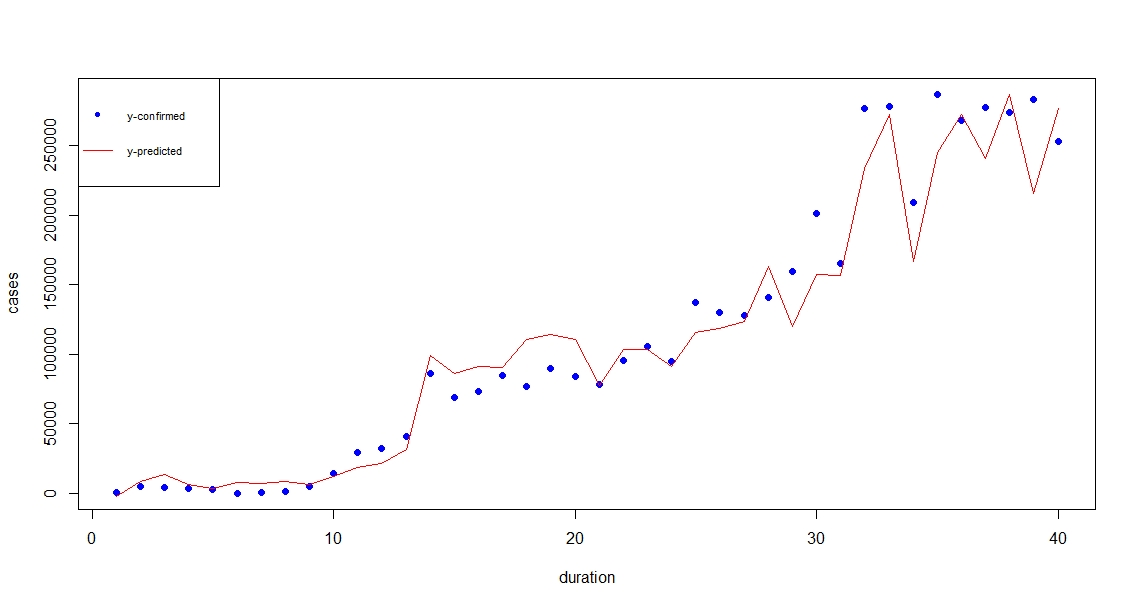
\includegraphics{images_for_report/confirmed_vs_predicted.jpeg}
\caption{confirmed\_vs\_predicted.jpeg}
\end{figure}

\begin{figure}
\centering
\includegraphics{attachment:diagnostic_plot_LRmodel.jpeg}
\caption{diagnostic\_plot\_LRmodel.jpeg}
\end{figure}

\hypertarget{consideration-on-the-incidence}{%
\subsubsection{Consideration on the
incidence}\label{consideration-on-the-incidence}}

In order to infer whether different countries had different death
incidence we did a two sided t.test for the incidence considering all
the possible combinations between the countries (total of N*(N-1)/2 )
and then stored the p-value in another dataframe. We then calculated the
mean of all the p-values obtaining \textbf{0.6912598}. The
Null-Hypothesis, being that the death incidences are differents, can not
be rejected.

\hypertarget{conclusions-further-steps}{%
\section{Conclusions \& Further Steps}\label{conclusions-further-steps}}

\hypertarget{conclusions}{%
\subsection{Conclusions:}\label{conclusions}}

After cleaning and preprocessing the data, looking carefully into the
relationship between all predictors as well as their relationships with
the outcome variables, we went ahead with the analysis of the data.
First, we wanted to use this data to predict the number of confirmed
cases based on chosen predictors. After going through a deep analysis of
different models \& comparing them with respect to different metrics, we
concluded that the best performing model was the following:

● Outcome variable: Global\_conf

● Predictors: Recovery and Death as 2nd degree polynomial

This model yielded us with an adjusted R-squared value of 95\% which we
found to be an indicator of an accurate prediction for future values.

\hypertarget{further-steps}{%
\subsection{Further Steps:}\label{further-steps}}

Some further steps that should be considered is the growth rate of the
global confirmed cases. As seen in our data, there was a significant
increase in the confirmed cases in between the dates 23rd January 2020
to 24th August 2020 which has an exponential increase considering the
precautions and other measures taken to prevent the spreading. This
number may increase for upcoming days considering no availability of
vaccine in near future.

The growth rate may be affected by many factors irrespective of
countries like age, immune related disease, cardiovascular disease,
pollution factor, diets, exercise habits and other personal hygiene
practices.

That is why we believed in considering the day to day analysis of data
across the globe considering the growth rate in order to predict more
accurately the number of confirmed cases. This will help make informed
decisions about how to take additional precautionary measures to prevent
the outbreak spreading.

\hypertarget{technical-appendix}{%
\section{Technical Appendix}\label{technical-appendix}}

\hypertarget{regression-assumptions}{%
\subsubsection{1. Regression assumptions
:}\label{regression-assumptions}}

Linear regression makes several assumptions about the data, such as :

\textbf{1.1 Linearity of the data:} The relationship between the
predictor (x) and the outcome (y) is assumed to be linear.

\textbf{1.2 Normality of residuals:} The residual errors are assumed to
be normally distributed.

\textbf{1.3 Homogeneity of residuals variance:} The residuals are
assumed to have a constant variance (homoscedasticity)

\textbf{1.4 Independence of residuals error terms.}

\hypertarget{residual-distribution}{%
\subsubsection{2. Residual Distribution:}\label{residual-distribution}}

The evidence that a linear regression model is appropriate comes in from
the residual vs fitted plot, whose values are randomly dispersed around
the horizontal axis, showing that the mean of residuals is really close
to 0. Moreover, the Normal Q-Q plot ensures that the distribution of
residuals is Gaussian one.

\hypertarget{regression-diagnostics}{%
\subsubsection{3. Regression diagnostics
:}\label{regression-diagnostics}}

The diagnostic plots show residuals in four different ways:

\textbf{3.1 Residuals vs Fitted.} Used to check the linear relationship
assumptions. A horizontal line, without distinct patterns is an
indication for a linear relationship, what is good.

\textbf{3.2 Normal Q-Q:} Used to examine whether the residuals are
normally distributed. It's good if residuals points follow the straight
dashed line. ``homogeneity of variance''

\textbf{3.3 Scale-Location (or Spread-Location):} Used to check the
homogeneity of variance of the residuals (homoscedasticity). Horizontal
line with equally spread points is a good indication of
homoscedasticity. This is not the case in our example, where we have a
heteroscedasticity problem.

\textbf{3.4 Residuals vs Leverage:} Used to identify influential cases,
that is extreme values that might influence the regression results when
included or excluded from the analysis. This plot will be described
further in the next sections.

\hypertarget{regression-model-evaluation-metrics}{%
\subsubsection{4. Regression Model Evaluation
Metrics:}\label{regression-model-evaluation-metrics}}

The MSE, MAE, RMSE, and R-Squared metrics are mainly used to evaluate
the prediction error rates and model performance in regression analysis.

\textbf{4.1 MAE (Mean absolute error):} It represents the difference
between the original and predicted values extracted by averaged the
absolute difference over the data set.
\[{\displaystyle \operatorname {MAE} ={\frac {1}{n}}\sum _{i=1}^{n}(Y_{i}-{\hat {Y_{i}}}).}\]

\textbf{4.2 MSE (Mean Squared Error):} It represents the difference
between the original and predicted values extracted by squared the
average difference over the data set.
\[{\displaystyle \operatorname {MSE} ={\frac {1}{n}}\sum _{i=1}^{n}(Y_{i}-{\hat {Y_{i}}})^{2}.}\]

\textbf{4.3 RMSE (Root Mean Squared Error):} It is the error rate by the
square root of MSE.

\[{\displaystyle \operatorname {RMSE} ={\sqrt{MSE}} = {\sqrt {\frac {1}{n}\sum _{i=1}^{n}(Y_{i}-{\hat {Y_{i}}})^{2}}}.}\]

where \(Y_{i}\) is the original value and \({\hat {Y_{i}}}\) is the
predicted one.

\textbf{4.4 R-squared (Coefficient of determination):} It represents the
coefficient of how well the values fit compared to the original values.
The value from 0 to 1 interpreted as percentages. The higher the value
is, the better the model is.

\textbf{4.5 Adjusted R-squared:} It is a model version of R-squared that
has been adjusted for the number of predictors in the model. It
increases only when an independent variable is significant and affects
the dependent variable.

Formula: where is the sample adj.R2 = 1 − (1 − R2){[}n − 1/n − (k +
1){]} n size and k is the number of independent variables in the
regression equation.

\textbf{4.6 p\_value:} A predictor that has a low p\_value
(\textless{}0.05) indicates that we should reject the null hypothesis.
In other words, a predictor that has a low p\_value is likely to be a
meaningful addition to our model because changes in the predictor's
value are related to changes in the response variable. Conversely, a
larger (insignificant) p\_value suggests that changes in the predictor
are not associated with changes in response.

\hypertarget{cross-validation}{%
\subsubsection{5. Cross Validation:}\label{cross-validation}}

The basic idea behind cross validation techniques, consists of dividing
the data into two sets:

\begin{enumerate}
\def\labelenumi{\alph{enumi}.}
\item
  The training set: 80\% random split used to build the model.
\item
  The validation (test) set: 20\% random split used to validate (test)
  the model by estimating the prediction error.
\end{enumerate}

In our case, we used random split cross validation, split the data into
2 subsets. Cross Validation is a robust method for estimating the
accuracy of a model.


    % Add a bibliography block to the postdoc
    
    
    
    \end{document}
